\documentclass[11pt,a4paper,]{article}
\usepackage{lmodern}

\usepackage{amssymb,amsmath}
\usepackage{ifxetex,ifluatex}
\usepackage{fixltx2e} % provides \textsubscript
\ifnum 0\ifxetex 1\fi\ifluatex 1\fi=0 % if pdftex
  \usepackage[T1]{fontenc}
  \usepackage[utf8]{inputenc}
\else % if luatex or xelatex
  \usepackage{unicode-math}
  \defaultfontfeatures{Ligatures=TeX,Scale=MatchLowercase}
\fi
% use upquote if available, for straight quotes in verbatim environments
\IfFileExists{upquote.sty}{\usepackage{upquote}}{}
% use microtype if available
\IfFileExists{microtype.sty}{%
\usepackage[]{microtype}
\UseMicrotypeSet[protrusion]{basicmath} % disable protrusion for tt fonts
}{}
\PassOptionsToPackage{hyphens}{url} % url is loaded by hyperref
\usepackage[unicode=true]{hyperref}
\hypersetup{
            pdftitle={Expert advice from experts},
            pdfborder={0 0 0},
            breaklinks=true}
\urlstyle{same}  % don't use monospace font for urls
\usepackage{geometry}
\geometry{a4paper, centering, text={16cm,24cm}}
\usepackage[style=authoryear-comp,]{biblatex}
\addbibresource{references.bib}
\usepackage{color}
\usepackage{fancyvrb}
\newcommand{\VerbBar}{|}
\newcommand{\VERB}{\Verb[commandchars=\\\{\}]}
\DefineVerbatimEnvironment{Highlighting}{Verbatim}{commandchars=\\\{\}}
% Add ',fontsize=\small' for more characters per line
\usepackage{framed}
\definecolor{shadecolor}{RGB}{248,248,248}
\newenvironment{Shaded}{\begin{snugshade}}{\end{snugshade}}
\newcommand{\AlertTok}[1]{\textcolor[rgb]{0.94,0.16,0.16}{#1}}
\newcommand{\AnnotationTok}[1]{\textcolor[rgb]{0.56,0.35,0.01}{\textbf{\textit{#1}}}}
\newcommand{\AttributeTok}[1]{\textcolor[rgb]{0.77,0.63,0.00}{#1}}
\newcommand{\BaseNTok}[1]{\textcolor[rgb]{0.00,0.00,0.81}{#1}}
\newcommand{\BuiltInTok}[1]{#1}
\newcommand{\CharTok}[1]{\textcolor[rgb]{0.31,0.60,0.02}{#1}}
\newcommand{\CommentTok}[1]{\textcolor[rgb]{0.56,0.35,0.01}{\textit{#1}}}
\newcommand{\CommentVarTok}[1]{\textcolor[rgb]{0.56,0.35,0.01}{\textbf{\textit{#1}}}}
\newcommand{\ConstantTok}[1]{\textcolor[rgb]{0.00,0.00,0.00}{#1}}
\newcommand{\ControlFlowTok}[1]{\textcolor[rgb]{0.13,0.29,0.53}{\textbf{#1}}}
\newcommand{\DataTypeTok}[1]{\textcolor[rgb]{0.13,0.29,0.53}{#1}}
\newcommand{\DecValTok}[1]{\textcolor[rgb]{0.00,0.00,0.81}{#1}}
\newcommand{\DocumentationTok}[1]{\textcolor[rgb]{0.56,0.35,0.01}{\textbf{\textit{#1}}}}
\newcommand{\ErrorTok}[1]{\textcolor[rgb]{0.64,0.00,0.00}{\textbf{#1}}}
\newcommand{\ExtensionTok}[1]{#1}
\newcommand{\FloatTok}[1]{\textcolor[rgb]{0.00,0.00,0.81}{#1}}
\newcommand{\FunctionTok}[1]{\textcolor[rgb]{0.00,0.00,0.00}{#1}}
\newcommand{\ImportTok}[1]{#1}
\newcommand{\InformationTok}[1]{\textcolor[rgb]{0.56,0.35,0.01}{\textbf{\textit{#1}}}}
\newcommand{\KeywordTok}[1]{\textcolor[rgb]{0.13,0.29,0.53}{\textbf{#1}}}
\newcommand{\NormalTok}[1]{#1}
\newcommand{\OperatorTok}[1]{\textcolor[rgb]{0.81,0.36,0.00}{\textbf{#1}}}
\newcommand{\OtherTok}[1]{\textcolor[rgb]{0.56,0.35,0.01}{#1}}
\newcommand{\PreprocessorTok}[1]{\textcolor[rgb]{0.56,0.35,0.01}{\textit{#1}}}
\newcommand{\RegionMarkerTok}[1]{#1}
\newcommand{\SpecialCharTok}[1]{\textcolor[rgb]{0.00,0.00,0.00}{#1}}
\newcommand{\SpecialStringTok}[1]{\textcolor[rgb]{0.31,0.60,0.02}{#1}}
\newcommand{\StringTok}[1]{\textcolor[rgb]{0.31,0.60,0.02}{#1}}
\newcommand{\VariableTok}[1]{\textcolor[rgb]{0.00,0.00,0.00}{#1}}
\newcommand{\VerbatimStringTok}[1]{\textcolor[rgb]{0.31,0.60,0.02}{#1}}
\newcommand{\WarningTok}[1]{\textcolor[rgb]{0.56,0.35,0.01}{\textbf{\textit{#1}}}}
\usepackage{longtable,booktabs}
% Fix footnotes in tables (requires footnote package)
\IfFileExists{footnote.sty}{\usepackage{footnote}\makesavenoteenv{long table}}{}
\usepackage{graphicx,grffile}
\makeatletter
\def\maxwidth{\ifdim\Gin@nat@width>\linewidth\linewidth\else\Gin@nat@width\fi}
\def\maxheight{\ifdim\Gin@nat@height>\textheight\textheight\else\Gin@nat@height\fi}
\makeatother
% Scale images if necessary, so that they will not overflow the page
% margins by default, and it is still possible to overwrite the defaults
% using explicit options in \includegraphics[width, height, ...]{}
\setkeys{Gin}{width=\maxwidth,height=\maxheight,keepaspectratio}
\IfFileExists{parskip.sty}{%
\usepackage{parskip}
}{% else
\setlength{\parindent}{0pt}
\setlength{\parskip}{6pt plus 2pt minus 1pt}
}
\setlength{\emergencystretch}{3em}  % prevent overfull lines
\providecommand{\tightlist}{%
  \setlength{\itemsep}{0pt}\setlength{\parskip}{0pt}}
\setcounter{secnumdepth}{5}

% set default figure placement to htbp
\makeatletter
\def\fps@figure{htbp}
\makeatother


\title{Expert advice from experts}

%% MONASH STUFF

%% CAPTIONS
\RequirePackage{caption}
\DeclareCaptionStyle{italic}[justification=centering]
 {labelfont={bf},textfont={it},labelsep=colon}
\captionsetup[figure]{style=italic,format=hang,singlelinecheck=true}
\captionsetup[table]{style=italic,format=hang,singlelinecheck=true}


%% FONT
\RequirePackage{bera}
\RequirePackage[charter,expert,sfscaled]{mathdesign}
\RequirePackage{fontawesome}

%% HEADERS AND FOOTERS
\RequirePackage{fancyhdr}
\pagestyle{fancy}
\rfoot{\Large\sffamily\raisebox{-0.1cm}{\textbf{\thepage}}}
\makeatletter
\lhead{\textsf{\expandafter{\@title}}}
\makeatother
\rhead{}
\cfoot{}
\setlength{\headheight}{15pt}
\renewcommand{\headrulewidth}{0.4pt}
\renewcommand{\footrulewidth}{0.4pt}
\fancypagestyle{plain}{%
\fancyhf{} % clear all header and footer fields
\fancyfoot[C]{\sffamily\thepage} % except the center
\renewcommand{\headrulewidth}{0pt}
\renewcommand{\footrulewidth}{0pt}}

%% MATHS
\RequirePackage{bm,amsmath}
\allowdisplaybreaks

%% GRAPHICS
\RequirePackage{graphicx}
\setcounter{topnumber}{2}
\setcounter{bottomnumber}{2}
\setcounter{totalnumber}{4}
\renewcommand{\topfraction}{0.85}
\renewcommand{\bottomfraction}{0.85}
\renewcommand{\textfraction}{0.15}
\renewcommand{\floatpagefraction}{0.8}


%\RequirePackage[section]{placeins}

%% SECTION TITLES


%% SECTION TITLES
\RequirePackage[compact,sf,bf]{titlesec}
\titleformat*{\section}{\Large\sf\bfseries\color[rgb]{0.7,0,0}}
\titleformat*{\subsection}{\large\sf\bfseries\color[rgb]{0.7,0,0}}
\titleformat*{\subsubsection}{\sf\bfseries\color[rgb]{0.7,0,0}}
\titlespacing{\section}{0pt}{2ex}{.5ex}
\titlespacing{\subsection}{0pt}{1.5ex}{0ex}
\titlespacing{\subsubsection}{0pt}{.5ex}{0ex}


%% TITLE PAGE
\def\Date{\number\day}
\def\Month{\ifcase\month\or
 January\or February\or March\or April\or May\or June\or
 July\or August\or September\or October\or November\or December\fi}
\def\Year{\number\year}

%% LINE AND PAGE BREAKING
\sloppy
\clubpenalty = 10000
\widowpenalty = 10000
\brokenpenalty = 10000
\RequirePackage{microtype}

%% PARAGRAPH BREAKS
\setlength{\parskip}{1.4ex}
\setlength{\parindent}{0em}

%% HYPERLINKS
\RequirePackage{xcolor} % Needed for links
\definecolor{darkblue}{rgb}{0,0,.6}
\RequirePackage{url}

\makeatletter
\@ifpackageloaded{hyperref}{}{\RequirePackage{hyperref}}
\makeatother
\hypersetup{
     citecolor=0 0 0,
     breaklinks=true,
     bookmarksopen=true,
     bookmarksnumbered=true,
     linkcolor=darkblue,
     urlcolor=blue,
     citecolor=darkblue,
     colorlinks=true}

\usepackage[showonlyrefs]{mathtools}
\usepackage[no-weekday]{eukdate}

%% BIBLIOGRAPHY

\makeatletter
\@ifpackageloaded{biblatex}{}{\usepackage[style=authoryear-comp, backend=biber, natbib=true]{biblatex}}
\makeatother
\ExecuteBibliographyOptions{bibencoding=utf8,minnames=1,maxnames=3, maxbibnames=99,dashed=false,terseinits=true,giveninits=true,uniquename=false,uniquelist=false,doi=false, isbn=false,url=true,sortcites=false}

\DeclareFieldFormat{url}{\texttt{\url{#1}}}
\DeclareFieldFormat[article]{pages}{#1}
\DeclareFieldFormat[inproceedings]{pages}{\lowercase{pp.}#1}
\DeclareFieldFormat[incollection]{pages}{\lowercase{pp.}#1}
\DeclareFieldFormat[article]{volume}{\mkbibbold{#1}}
\DeclareFieldFormat[article]{number}{\mkbibparens{#1}}
\DeclareFieldFormat[article]{title}{\MakeCapital{#1}}
\DeclareFieldFormat[article]{url}{}
%\DeclareFieldFormat[book]{url}{}
%\DeclareFieldFormat[inbook]{url}{}
%\DeclareFieldFormat[incollection]{url}{}
%\DeclareFieldFormat[inproceedings]{url}{}
\DeclareFieldFormat[inproceedings]{title}{#1}
\DeclareFieldFormat{shorthandwidth}{#1}
%\DeclareFieldFormat{extrayear}{}
% No dot before number of articles
\usepackage{xpatch}
\xpatchbibmacro{volume+number+eid}{\setunit*{\adddot}}{}{}{}
% Remove In: for an article.
\renewbibmacro{in:}{%
  \ifentrytype{article}{}{%
  \printtext{\bibstring{in}\intitlepunct}}}

\AtEveryBibitem{\clearfield{month}}
\AtEveryCitekey{\clearfield{month}}

\makeatletter
\DeclareDelimFormat[cbx@textcite]{nameyeardelim}{\addspace}
\makeatother

\author{\sf\Large\textbf{ Marie Curie}\\ {\sf\large Nobel Prize, PhD\\[0.5cm]} \sf\Large\textbf{ Pierre Curie}\\ {\sf\large Nobel Prize, PhD\\[0.5cm]}}

\date{\sf\Date~\Month~\Year}
\makeatletter
\lfoot{\sf Curie, Curie: \@date}
\makeatother


%%%% PAGE STYLE FOR FRONT PAGE OF REPORTS

\makeatletter
\def\organization#1{\gdef\@organization{#1}}
\def\telephone#1{\gdef\@telephone{#1}}
\def\email#1{\gdef\@email{#1}}
\makeatother
  \organization{Acme Corporation}

  \def\name{Department of\newline Econometrics \&\newline Business Statistics}

  \telephone{(03) 9905 2478}

  \email{BusEco-Econometrics@monash.edu}

\def\webaddress{\url{http://buseco.monash.edu/ebs/consulting/}}
\def\abn{12 377 614 012}
\def\logo{
\includegraphics[width=6cm]{MBSportrait}}
\def\extraspace{\vspace*{1.6cm}}
\makeatletter
\def\contactdetails{\faicon{phone} & \@telephone \\
                    \faicon{envelope} & \@email}
\makeatother

%%%% FRONT PAGE OF REPORTS

\def\reporttype{Report for}

\long\def\front#1#2#3{
\newpage
\begin{singlespacing}
\thispagestyle{empty}
\vspace*{-1.4cm}
\hspace*{-1.4cm}
\hbox to 16cm{
  \hbox to 6.5cm{\vbox to 14cm{\vbox to 25cm{
    \logo
    \vfill
    \parbox{6.3cm}{\raggedright
      \sf\color[rgb]{0.00,0.00,0.70}
      {\large\textbf{\name}}\par
      \vspace{.7cm}
      \tabcolsep=0.12cm\sf\small
      \begin{tabular}{@{}ll@{}}\contactdetails
      \end{tabular}
      \vspace*{0.3cm}\par
      ABN: \abn\par
    }
  }\vss}\hss}
  \hspace*{0.2cm}
  \hbox to 1cm{\vbox to 14cm{\rule{1pt}{26.8cm}\vss}\hss\hfill}
  \hbox to 10cm{\vbox to 14cm{\vbox to 25cm{
      \vspace*{3cm}\sf\raggedright
      \parbox{11cm}{\sf\raggedright\baselineskip=1.2cm
         \fontsize{24.88}{30}\color[rgb]{0.70,0.00,0.00}\sf\textbf{#1}}
      \par
      \vfill
      \large
      \vbox{\parskip=0.8cm #2}\par
      \vspace*{2cm}\par
      \reporttype\\[0.3cm]
      \hbox{#3}%\\[2cm]\
      \vspace*{1cm}
      {\large\sf\textbf{\Date~\Month~\Year}}
   }\vss}
  }}
\end{singlespacing}
\newpage
}

\makeatletter
\def\titlepage{\front{\expandafter{\@title}}{\@author}{\@organization}}
\makeatother

\usepackage{setspace}
\setstretch{1.5}

%% Any special functions or other packages can be loaded here.


\begin{document}
\titlepage

\begin{Shaded}
\begin{Highlighting}[]
\NormalTok{Miss\_tidy \textless{}{-}}\StringTok{ }\KeywordTok{vis\_miss}\NormalTok{(hotels, }\DataTypeTok{warn\_large\_data =}\OtherTok{FALSE}\NormalTok{) }\CommentTok{\# Check mssing value }
\NormalTok{Miss\_tidy}
\end{Highlighting}
\end{Shaded}

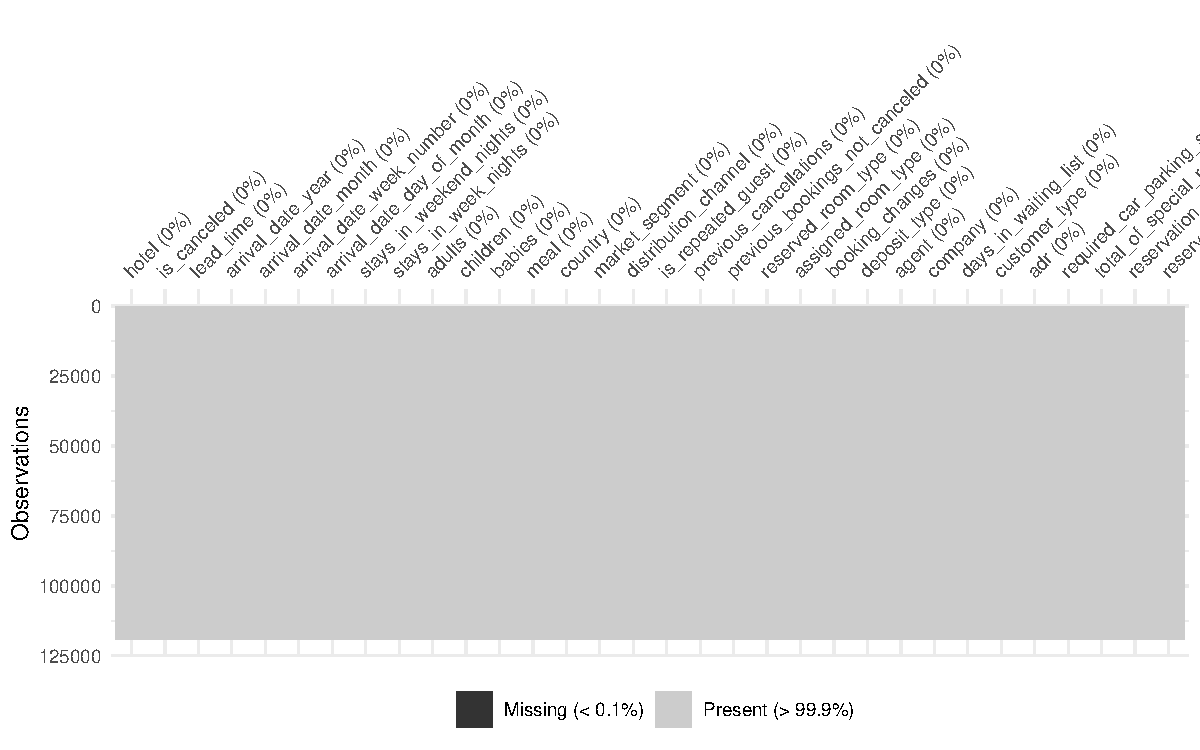
\includegraphics{tidy_files/figure-latex/check NA-1.pdf}

\begin{Shaded}
\begin{Highlighting}[]
\NormalTok{hotel \textless{}{-}}\StringTok{ }\KeywordTok{na.omit}\NormalTok{(hotels)}
\end{Highlighting}
\end{Shaded}

\begin{Shaded}
\begin{Highlighting}[]
\NormalTok{hotel \textless{}{-}}\StringTok{ }\NormalTok{hotel }\OperatorTok{\%\textgreater{}\%}\StringTok{ }\KeywordTok{mutate}\NormalTok{(}
    \DataTypeTok{arr\_date\_month =} \KeywordTok{case\_when}\NormalTok{(   }\CommentTok{\# change Month to the numeric }
\NormalTok{    arrival\_date\_month}\OperatorTok{==}\StringTok{"January"} \OperatorTok{\textasciitilde{}}\StringTok{ }\DecValTok{01}\NormalTok{,}
\NormalTok{    arrival\_date\_month}\OperatorTok{==}\StringTok{"February"} \OperatorTok{\textasciitilde{}}\StringTok{ }\DecValTok{02}\NormalTok{,}
\NormalTok{    arrival\_date\_month}\OperatorTok{==}\StringTok{"March"} \OperatorTok{\textasciitilde{}}\StringTok{ }\DecValTok{03}\NormalTok{,}
\NormalTok{    arrival\_date\_month}\OperatorTok{==}\StringTok{"April"} \OperatorTok{\textasciitilde{}}\StringTok{ }\DecValTok{04}\NormalTok{,}
\NormalTok{    arrival\_date\_month}\OperatorTok{==}\StringTok{"May"} \OperatorTok{\textasciitilde{}}\StringTok{ }\DecValTok{05}\NormalTok{,}
\NormalTok{    arrival\_date\_month}\OperatorTok{==}\StringTok{"June"} \OperatorTok{\textasciitilde{}}\StringTok{ }\DecValTok{06}\NormalTok{,}
\NormalTok{    arrival\_date\_month}\OperatorTok{==}\StringTok{"July"} \OperatorTok{\textasciitilde{}}\StringTok{ }\DecValTok{07}\NormalTok{,}
\NormalTok{    arrival\_date\_month}\OperatorTok{==}\StringTok{"August"} \OperatorTok{\textasciitilde{}}\StringTok{ }\DecValTok{08}\NormalTok{,}
\NormalTok{    arrival\_date\_month}\OperatorTok{==}\StringTok{"September"} \OperatorTok{\textasciitilde{}}\StringTok{ }\DecValTok{09}\NormalTok{,}
\NormalTok{    arrival\_date\_month}\OperatorTok{==}\StringTok{"October"} \OperatorTok{\textasciitilde{}}\StringTok{ }\DecValTok{10}\NormalTok{,}
\NormalTok{    arrival\_date\_month}\OperatorTok{==}\StringTok{"November"} \OperatorTok{\textasciitilde{}}\StringTok{ }\DecValTok{11}\NormalTok{,}
\NormalTok{    arrival\_date\_month}\OperatorTok{==}\StringTok{"December"} \OperatorTok{\textasciitilde{}}\StringTok{ }\DecValTok{12}\NormalTok{),}
    \DataTypeTok{country =} \KeywordTok{str\_replace}\NormalTok{(country, }\DataTypeTok{pattern =} \StringTok{"cn"}\NormalTok{, }\DataTypeTok{replacement =} \StringTok{"chn"}\NormalTok{), }\CommentTok{\# replace China pattern}
    \DataTypeTok{deposit =} \KeywordTok{case\_when}\NormalTok{(deposit\_type }\OperatorTok{==}\StringTok{ "No Deposit"}\OperatorTok{\textasciitilde{}}\DecValTok{0}\NormalTok{,            }\CommentTok{\# Change deposit as binary numeric}
\NormalTok{                        deposit\_type }\OperatorTok{==}\StringTok{ "Non Refund"}\OperatorTok{\textasciitilde{}}\DecValTok{1}\NormalTok{,}
\NormalTok{                         deposit\_type }\OperatorTok{==}\StringTok{ "Refundable"}\OperatorTok{\textasciitilde{}}\DecValTok{2}\NormalTok{),}
   \DataTypeTok{arrival\_time=}\KeywordTok{paste}\NormalTok{(arrival\_date\_year,}
\NormalTok{                      arrival\_date\_month,}
\NormalTok{                      arrival\_date\_day\_of\_month,}
                      \DataTypeTok{sep=}\StringTok{"{-}"}\NormalTok{))}
\NormalTok{  sec\_mute \textless{}{-}}\StringTok{ }\NormalTok{hotel }\OperatorTok{\%\textgreater{}\%}\StringTok{ }\KeywordTok{mutate}\NormalTok{(}\DataTypeTok{Country =} \KeywordTok{countrycode}\NormalTok{(}\DataTypeTok{sourcevar =}\NormalTok{ country,              }\CommentTok{\# According the country code to find the country full name}
                                      \DataTypeTok{origin =} \StringTok{"iso3c"}\NormalTok{,}
                                      \DataTypeTok{destination =} \StringTok{"country.name"}\NormalTok{),}
          \DataTypeTok{reservation\_status\_date=}\KeywordTok{ymd}\NormalTok{(reservation\_status\_date),}
         \DataTypeTok{arrival\_time=}\KeywordTok{ymd}\NormalTok{(arrival\_time)) }
\end{Highlighting}
\end{Shaded}

\begin{Shaded}
\begin{Highlighting}[]
\NormalTok{Miss \textless{}{-}}\StringTok{ }\KeywordTok{sapply}\NormalTok{(hotels, }\ControlFlowTok{function}\NormalTok{(x) }\KeywordTok{sum}\NormalTok{(}\KeywordTok{is.na}\NormalTok{(x))) }\CommentTok{\# Check mssing value }
\NormalTok{Miss}
\end{Highlighting}
\end{Shaded}

\begin{verbatim}
##                          hotel                    is_canceled 
##                              0                              0 
##                      lead_time              arrival_date_year 
##                              0                              0 
##             arrival_date_month       arrival_date_week_number 
##                              0                              0 
##      arrival_date_day_of_month        stays_in_weekend_nights 
##                              0                              0 
##           stays_in_week_nights                         adults 
##                              0                              0 
##                       children                         babies 
##                              4                              0 
##                           meal                        country 
##                              0                              0 
##                 market_segment           distribution_channel 
##                              0                              0 
##              is_repeated_guest         previous_cancellations 
##                              0                              0 
## previous_bookings_not_canceled             reserved_room_type 
##                              0                              0 
##             assigned_room_type                booking_changes 
##                              0                              0 
##                   deposit_type                          agent 
##                              0                              0 
##                        company           days_in_waiting_list 
##                              0                              0 
##                  customer_type                            adr 
##                              0                              0 
##    required_car_parking_spaces      total_of_special_requests 
##                              0                              0 
##             reservation_status        reservation_status_date 
##                              0                              0
\end{verbatim}

\begin{Shaded}
\begin{Highlighting}[]
\NormalTok{vis\_tidy \textless{}{-}}\StringTok{ }\KeywordTok{vis\_miss}\NormalTok{(sec\_mute, }\DataTypeTok{warn\_large\_data =}\OtherTok{FALSE}\NormalTok{)}
\NormalTok{vis\_tidy}
\end{Highlighting}
\end{Shaded}

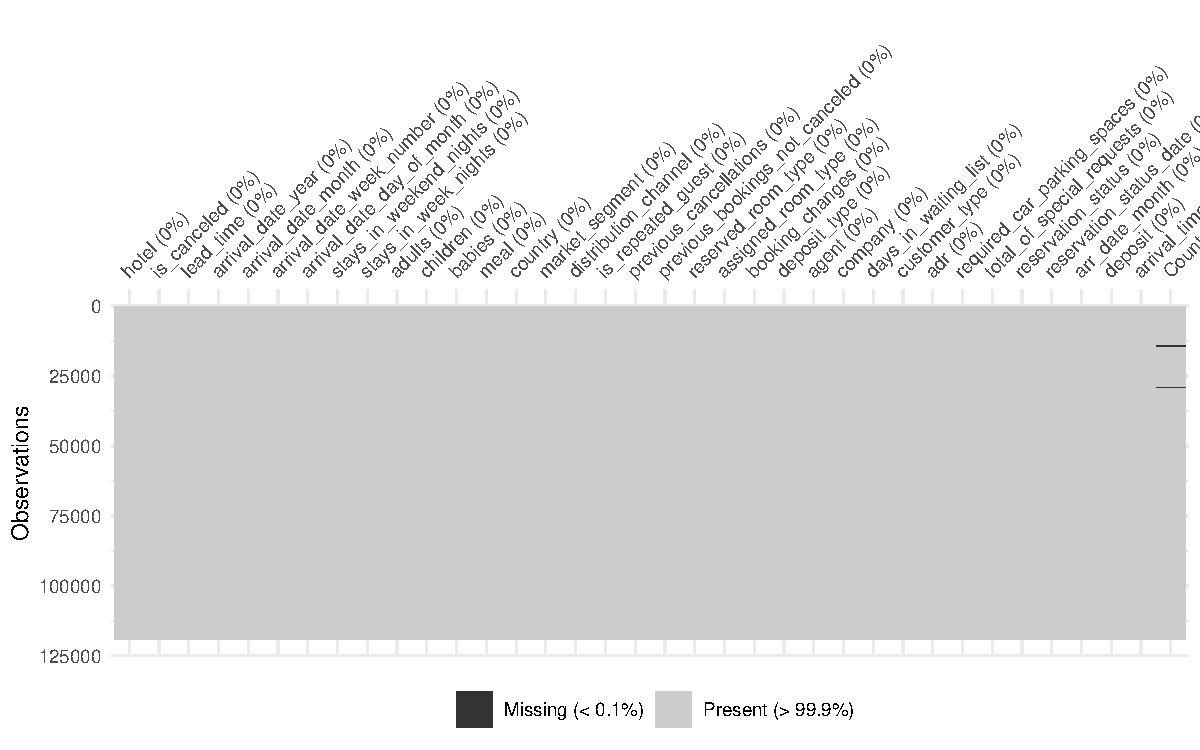
\includegraphics{tidy_files/figure-latex/sectidy-1.pdf}

\begin{Shaded}
\begin{Highlighting}[]
\NormalTok{sec\_mute \textless{}{-}}\StringTok{ }\NormalTok{sec\_mute  }\OperatorTok{\%\textgreater{}\%}\StringTok{ }\NormalTok{dplyr}\OperatorTok{::}\KeywordTok{select}\NormalTok{(}\OperatorTok{{-}}\NormalTok{market\_segment,}
                               \OperatorTok{{-}}\NormalTok{distribution\_channel,}
                               \OperatorTok{{-}}\NormalTok{deposit\_type,}
                               \OperatorTok{{-}}\NormalTok{agent,}
                               \OperatorTok{{-}}\NormalTok{company) }
\end{Highlighting}
\end{Shaded}

\begin{Shaded}
\begin{Highlighting}[]
\NormalTok{final \textless{}{-}}\StringTok{ }\KeywordTok{na.omit}\NormalTok{(sec\_mute)  }\CommentTok{\# Delete the missing country observations}
\end{Highlighting}
\end{Shaded}


\printbibliography

\end{document}
